\documentclass[output=paper]{langscibook}
\ChapterDOI{10.5281/zenodo.18845924}
\author{Eugenio Goria\orcid{}\affiliation{University of Turin} and Kate Bellamy\orcid{}\affiliation{Leiden University}}
\title[Code-mixing and language change]{Code-mixing and language change: Evidence from Spanish nouns in heritage Piedmontese}
\abstract{In this paper we provide a qualitative and quantitative analysis of Argentinian Spanish noun insertion in Heritage Piedmontese (\textsc{hp} henceforth), an Italo-Romance minority language that is also spoken in Argentina. Despite language shift towards the national language, Spanish, \textsc{hp} continues to be used in a number of culturally relevant situations. In these situations, where code-mixing is commonplace, \textsc{hp} is usually the matrix language of bilingual interaction. We show that mixed noun phrases (NP's) display considerable variation in the realisation of gender and number marking, despite a certain amount of morphological and phonological congruence between the nominal systems of the two languages. Our analysis is based on a sample of five hours of speech, extracted from a larger corpus of interviews and conversations in \textsc{hp} collected between 2019 and 2022 in the framework of the \textsc{pilar} - Piedmontese Language in Argentina project. Building on previous taxonomies, we identify three main types of code-mixing in the \textsc{hp}{}-Spanish data: (i) alternations, where a Spanish NP is part of a code-switch spanning over several constituents; (ii) maximal insertions, involving a Spanish embedded-language island; and (iii) minimal insertions, where a Spanish noun is inserted into a Piedmontese morphological structure, either as a bare stem or adopting Piedmontese morphology. We identified 318 mixed NP's, of which the bare stem type is the most common. On the basis of a comparison of gender and number marking in Spanish and Piedmontese, we demonstrate that the observed types of code-mixing are mostly predicted by typological similarities and differences between the two languages involved. Also new patterns of number marking have emerged from the analysis, which suggest a new hypothesis on the relationship between code-mixing and language change.}
\IfFileExists{../localcommands.tex}{
  \addbibresource{../localbibliography.bib}
  \usepackage{tabularx,multicol}
\usepackage{url}
\urlstyle{same}

 
\usepackage{langsci-optional}
\usepackage{langsci-lgr}
\usepackage{langsci-gb4e}

\usepackage{multirow}
\usepackage{cleveref}
\usepackage{subfigure}
\usepackage{langsci-branding}

  \input{../localcommands} 
  \input{../localhyphenation} 
  \togglepaper[2]%%chapternumber
}{}

\begin{document}
\maketitle 
%\shorttitlerunninghead{}%%use this for an abridged title in the page headers


\section{Introduction}\label{sec:goria:1}

In this paper we analyse code-mixing\footnote{The term ‘code-mixing’ is used here following \citet{Auer1999} as a type of bilingual speech phenomenon where the juxtaposition between two (or more) codes in the same discourse does not bear any pragmatic meaning. See \sectref{sec:goria:2}.} in the Piedmontese-speaking community in Argentina. Piedmontese is an Italo-Romance minority language, spoken in the northwestern Italian region of Piedmont (Italian: Piemonte). It does not have official status in Italian law, and has undergone normative standardisation only to a certain degree (see \citealt{Regis2013,RegisRivoirainpress}, for a more detailed discussion). Piedmontese was regularly used, especially in informal situations, until the first half of the twentieth century, but is currently undergoing language shift towards Standard Italian along the well-described path from spoken diglossia to diaglossia \citep{Auer2005}, or ‘dilalia’ \citep{Berruto2012}. This shift describes a pattern in the evolution of linguistic repertoires that is common to most European countries: national standards, after starting out as H[igh] varieties in a diglossic situation, and thus almost exclusively confined to written uses, increasingly extend to the L[ow] domains, typical of spoken vernaculars, eventually becoming the main language within the household. A case in point is Standard Italian, which evolved from the status of an almost exclusively written to a spoken national language throughout the twentieth century, due to social and historical reasons, such as the introduction of compulsory primary education, the diffusion of Italian-speaking television, and internal migrations (\citealt{Mauro1963}). This resulted in a new configuration of the linguistic repertoire, where Piedmontese and the other Romance vernaculars spoken in Italy compete with the national language even in the most familiar and informal domains, thereby reducing the vernaculars to optional codes.\footnote{Differences between Auer’s notion of ‘diaglossia’ and Berruto’s ‘dilalia’ concern the status of the \textsc{l} variety, which is fundamentally a regiolect of \textsc{h} in Auer’s account, but a separate linguistic system functionally subordinated to \textsc{h} (that is, a minority language) in Berruto’s account.}

As an effect of Italian emigration, and especially during the period between the end of the nineteenth century and the outbreak of World War I, Piedmontese also came to be spoken outside of Italy, and particularly in Argentina, where the socio-political, as well as territorial conditions were favourable to its retention among the early migrants, as well as by their descendants (see \citealt{Giolitto2000,Giolitto2010,giolitto_palabras_2016,Goria2015,Goria2021,Doglioli2022}). We will refer to this variety throughout this paper as Heritage Piedmontese (\textsc{hp}), because both its linguistic features and the social conditions in which it is spoken reflect the typical features of heritage languages. We thus follow Jason Rothman’s definition of a heritage language, whereby:

\begin{quote}
A language qualifies as a heritage language if it is a language spoken at home or otherwise readily available to young children, and crucially this language is not a dominant language of the larger (national) society […] the heritage language is acquired on the basis of an interaction with naturalistic input and whatever in-born linguistic mechanisms are at play in any instance of child language acquisition. Differently [from monolingual acquisition], there is the possibility that quantitative and qualitative differences in heritage language input, influence of the societal majority language and differences in literacy and formal education can result in what on the surface seems to be arrested development of the heritage language or attrition in adult bilingual knowledge (\citealt{Rothman2009}: 156)
\end{quote}

Based on recent research on heritage languages (see, e.g., \citealt{BenmamounEtAl2013,Nagy2017,Polinsky2018,AalberseEtAl2019,GoriaDiSalvo2023}) we may thus expect Heritage Piedmontese to be shaped on the one hand by acquisitional factors, and on the other hand by contact with local Spanish as the dominant language in society.\footnote{A third dimension in this respect would be ‘internal’ contact between different varieties of Piedmontese, with the formation of a migrant koiné (see \citealt{Kerswill2006}) as one of the possible outcomes. The possibility is discussed in \citet{CerrutiEtAlinpress} and will not be further discussed here.}  Indeed, given the long-term contact with Spanish and its resulting bilingualism, it is perhaps unsurprising that many individuals, especially those in the provinces of Córdoba and Santa Fé, where Piedmontese migration has been particularly intensive, use both of their languages in the same conversation, sentence or phrase. We will refer to this practice as ‘code-mixing’; since the same term has been used by different authors and in different theoretical frameworks, we will follow, more specifically, the distinction made by \citet{Auer1999,Auer2014}, where code-mixing (as opposed to code-switching) is a type of bilingual speech where two languages are juxtaposed in discourse in a patterned way, and which is also often globally meaningful as a marker of mixed social identities (see also Footnote 1).

The rest of this chapter is structured as follows. In \sectref{sec:goria:2}, we discuss our approach to code-mixing and introduce the categories for classifying nominal insertion that were used in this study. In \sectref{sec:goria:3} we provide some general context on \textsc{hp} in Argentina, and we introduce the data and methods that were used for this paper. In \sectref{sec:goria:4}, based on a comparison of nominal inflection in \textsc{hp} and Spanish, we discuss our research questions and predictions. Results are presented in \sectref{sec:goria:5}, and in \sectref{sec:goria:6} we draw some conclusions and directions for future research.

\section{On code-mixing}\label{sec:goria:2}

Code-mixing, or language mixing, constitutes the “juxtaposition of two languages in which the use of two languages is meaningful (to participants) not in a local but only in a more global sense, that is, when seen as a recurrent pattern” \citep[310]{Auer1999}. Within this framework, code-mixing is opposed to code-switching as the latter reflects the strategic use of multiple languages in interaction and is typically associated with discourse-related or participant-related functions.

Code-mixing may be insertional in nature, where an element or elements from one language may be “inserted” into a main, or matrix, language (see also \citealt{Myers-Scotton1993duelling,Myers-Scotton2002,Muysken2000}); or it may be alternational, where (short) stretches of one language are juxtaposed with stretches of the other (or others), making it difficult to define a matrix language (see also \citealt{Muysken2000}, who indeed refers to this as “alternation”).\footnote{\citegen{Muysken2000} typology includes a third type of mixing, that is, 'congruent lexicalisation'. This implies the presence of a shared syntactic structure that complies with the abstract rules of both languages, and is filled with lexical items from either language giving rise to rather complex switches. Since this paper mostly deals with insertion, we did not consider this third type.} Typical examples of alternation and insertion are given in examples \REF{ex:goria:1} and \REF{ex:goria:2}--\REF{ex:goria:3} respectively. All examples are from the first author’s corpus, unless otherwise stated; as a convention, throughout the paper we will use lower-case for Piedmontese and capitals for Spanish.

\ea\label{ex:goria:1}
  \gll \textsc{entonces}, a=smij-a che a=l'=han brusa=se ij \textsc{papel} \textsc{en} \textsc{la} \textsc{aduana}\\
  so \textsc{3sg}=look-\textsc{3sg} that  \textsc{3sg}=\textsc{clit}=have:\textsc{3pl}  burn=\textsc{refl} the:\textsc{m.pl} papers in the customs\\
  \glt ‘It looks like the documents were burnt at the customs’
\z

\ea\label{ex:goria:2}
  \gll j=er-o contadin da\_là \textsc{chacar}{}-é da\_sì\\
  \textsc{clit}=be-\textsc{3pl} peasant there peasant-\textsc{deriv} here\\
  \glt ‘They were peasants there and peasants here’
\z

\ea\label{ex:goria:3}
  \gll perché \textsc{mi} pare parl-o nen \textsc{la} \textsc{histori-a} \textsc{suy-a} en  piemonteis\\
  because my parent speak-\textsc{3pl} \textsc{neg} the:\textsc{f.sg} story(\textsc{f})-\textsc{sg}  \textsc{poss.3pl-f.sg} in Piedmontese\\
  \glt ‘Because my parents did (lit. do) not tell their story in Piedmontese’
\z

Based on \citeauthor{Muysken2000}'s (\citeyear{Muysken2000,Muysken2013}) taxonomy and further elaborations such as \citet{DeucharEtAl2007}, example \REF{ex:goria:1} represents a typical case of alternation, as the Spanish part of the sentence spans over several constituents and does not form a constituent itself. Rather it can be said that the sentence begins in Piedmontese and continues in Spanish. Examples \REF{ex:goria:2} and \REF{ex:goria:3} represent two different cases of insertion, which means that in both cases, Spanish nouns are inserted in an otherwise Piedmontese syntactic structure. In \REF{ex:goria:2} the speaker is referring to the fact that Piedmontese migrants in Argentina had a similar occupation before and after migration, but it was given a different name. So, the lexical morpheme of the Argentinian Spanish \textit{chacarero} ‘peasant’ is used in combination with the Piedmontese derivational morpheme \textit{{}-é} which typically forms agent nouns (e.g. \textit{verdur-a} ‘groceries’ > \textit{verdur-é} ‘greengrocer’).\footnote{The examples are from the first author’s personal knowledge.} According to \citet{Auer2014}, this constitutes a minimal insertion, as a single lexical morpheme from one language is embedded within the grammatical frame of another language. Conversely, in \REF{ex:goria:3} \textit{la historia suya} ‘their story’ (lit. ‘the story their’) constitutes a maximal insertion in Auer’s terms, as a full NP in Spanish is inserted into an otherwise Piedmontese clause, and follows the rules of Piedmontese. Not only does the inserted NP contain solely lexical material from the embedded language (that is, Spanish), but it is also internally constructed following the syntactic rules of Spanish: homeland Piedmontese would have a different word order in this construction, namely a prenominal possessive determiner and no definite article (e.g. \textit{sua stòria} ‘their story’). \citet{Auer2014} refers to these maximal insertions also as embedded-language islands, following \citet{Myers-Scotton2002}.

While the three code-mixing patterns described here appear to be easily distinguishable from each other, the interpretation of corpus data is not always so straightforward, and only in a few restricted cases is the distinction between the types categorical. Rather, most cases are best modelled as nodes on a continuum between insertion and alternation. Since the aim of this paper is to provide an analysis of nominal insertion in Heritage Piedmontese, we propose here a more fine-grained classification of insertional code-mixing that enables us to provide a more thorough analysis of this phenomenon. Thus, in order to classify the bilingual patterns identified in the corpus, we propose the categories that are summarised in \tabref{tab:goria:1}.

\begin{table}
\begin{tabularx}{\textwidth}{QQQr}
\lsptoprule
Extension of the switch & Label & Type of morphological marking within the Noun Phrase & Example no.\\
\midrule
{ > 1 constituent} & { Alternation} & { Spanish morphology} & { \REF{ex:goria:1}}\\
{ > 1 morpheme within the same constituent} & { Maximal insertion} & { Spanish morphology} & { \REF{ex:goria:3}, \REF{ex:goria:4}, \REF{ex:goria:5}}\\
{ only lexical morpheme} & { Minimal insertion} & { Bare stems} & { \REF{ex:goria:6}}\\
&  & { Matrix language inflection} & { \REF{ex:goria:2}, \REF{ex:goria:7}}\\
\lspbottomrule
\end{tabularx}
\caption{Criteria adopted for the categorisation of bilingual patterns}
\label{tab:goria:1}
\end{table}

Since we are relying on a corpus of interviews and data collected in situations of language revitalisation (see \sectref{sec:goria:3} for further discussion), \textsc{hp} tends to be firmly established as the base language in interaction and the matrix language in code-mixing. Based on this general consideration, we regarded as instances of alternation proper all the cases like \REF{ex:goria:1}, where multiple elements in Spanish, which do not form a syntactic constituent, are juxtaposed in otherwise \textsc{hp} discourse. Following \citet{Auer2014}, we then identified a major distinction between maximal and minimal insertions. Maximal insertion in our view includes all the bilingual patterns where more than one morpheme is involved from the embedded language, among which we identify at least: complex NPs, involving several words, for example determiners, adjectives etc., as in \REF{ex:goria:3}; lists and other types of syntactically heavy constituents, as in \REF{ex:goria:4}; and single inflected nouns retaining Spanish overt morphology, as in \REF{ex:goria:5}.

\ea%4
    \label{ex:goria:4}
    \gll prima fas-\textsc{íamo} \textsc{cosecha} e dòpo \textsc{tambo} \textsc{leche}\\
         before do-\textsc{impf}:\textsc{1pl} \textsc{harvest} and then   \textsc{dairy} \textsc{milk}\\
    \glt ‘In the past we used to do harvest, and then dairy farm, milk (products)’
\z % you might need an extra \z if this is the last of several subexamples

\ea%5
    \label{ex:goria:5}
    \gll soma part-ì quandi l'=oma program-à ël viagi ch- a vint \textsc{peso}{}-\textsc{s}\\
         be:\textsc{aux}.\textsc{pll} leave-\textsc{pp} when \textsc{clit}=have:\textsc{aux}.\textsc{1pl} program-\textsc{pp} the:\textsc{m.sg} travel that at twenty peso-\textsc{pl}\\
    \glt ‘We left when we planned our travel, that (one dollar was) twenty \textsc{pesos’}
\z % you might need an extra \z if this is the last of several subexamples

Finally, minimal insertions are represented by cases where only the lexical morpheme is inserted into the other-language grammatical frame. In the case of \textsc{hp}{}-Spanish code-mixing, this may consist of two different patterns. The first one is represented by the insertion of bare nouns, that is stems that have no overt morphological marking in the donor language (as is the case with Spanish singular nouns), or which are treated as invariables in bilingual discourse, thereby losing their morphological marking; consider example \REF{ex:goria:6}.

\ea%6
    \label{ex:goria:6}
    \gll ël pì cit dij \textsc{varón}\\
         the:\textsc{m.sg} more young of.the:\textsc{m}.\textsc{pl} male\\
    \glt ‘The youngest of the males’
\z % you might need an extra \z if this is the last of several subexamples

In \REF{ex:goria:6}, the Spanish word \textit{varón} ‘male’ is inserted into an \textsc{hp} clause without any plural morphology and is treated as an invariable noun, which, as will be shown in \sectref{sec:goria:4}, also complies with the rules of plural marking in homeland Piedmontese. The second type of minimal insertion consists of cases where inserted nouns are inflected with morphemes of the matrix language, as is the case in \REF{ex:goria:2}, as well as in \REF{ex:goria:7}, where the Spanish noun \textit{obra} ‘facility’ takes the Piedmontese plural marker \textit{{}-e} and is inflected as a Piedmontese noun.

\ea%7
    \label{ex:goria:7}
    \gll l’=ha fait tant-e \textsc{obr}{}-e\\
         \textsc{clit}=have:\textsc{aux}.\textsc{3sg}  do:\textsc{pp}  many-\textsc{f}.\textsc{pl} facility(\textsc{f})-\textsc{pl}\\
    \glt ‘He built several facilities’
\z % you might need an extra \z if this is the last of several subexamples

Before delving into the distribution of these code-mixing strategies in our data, we will first briefly present \textsc{hp} in more detail, since descriptions in English are still rather scarce.

\section{On Heritage Piedmontese}\label{sec:goria:3}
\subsection{On Piedmontese}

As stated in \sectref{sec:goria:1}, Piedmontese (ISO 639-3 pms) is a Gallo-Italic Italo-Romance variety predominantly spoken as a minority language within the Piedmont region, in the northwest of Italy. While it is not fully recognised as a minority language by Italian law, several bottom-up actions have been taken for its protection and revitalisation, especially by local scholars and private institutions. Not unlike most Italo-Romance varieties, Piedmontese was the main language of oral communication in Piedmont until the first half of the 20th century, when Standard Italian started spreading across the population, in schools and through other widespread means of communication. Currently, Piedmontese is endangered, due to language shift towards Italian; it is still spoken especially in rural areas of Piedmont, almost exclusively in informal and familiar domains and alongside (or in competition with) Italian. As discussed by \citet {Regis2011,Regis2013,RegisRivoirainpress}, among others, there is considerable sub-regional variation in spoken Piedmontese, but the dialect from the capital city of Piedmont, Turin, enjoys particular prestige and has provided a basis for (partial) standardisation, as well as for the elaboration of a written norm (\citealt{BreroBertodatti1988}).

Piedmontese migration to Argentina began during the economic crisis that followed the unification of Italy in 1861. Analysing historical demographic accounts, historians (see \citealt{Nascimbene1987}) identify a north-western phase in Italian migration to Argentina, approximately between the last decades of the 19th century and the outbreak of the First World War in 1914. In this period, the majority of emigrants arriving in Argentina were Piedmontese agricultural workers. The arrival of workforce from Italy, and Europe in general, was encouraged by the Argentinian government, as a means to reinforce the agricultural exploitation of the grasslands in the provinces of Córdoba and Santa Fe, which soon were named \textit{la pampa gringa} (lit. ‘the prairie of the gringos’\footnote{\textit{Gringo} is a term with various connotations in Latin American countries; in Argentina it normally refers to a European immigrant.}). As emerges from \citegen{Giolitto2010} account, the typical settlement in this period was represented by a system of newly founded agricultural colonies, mostly inhabited by Piedmontese immigrants. Due to the distance and relative isolation from larger urban settlements, as well as to local self-administered schools, Piedmontese continued being spoken in these communities, and was even passed on to migrants from other regions or other European countries. Thus, language shift towards Spanish occurred at a much slower pace compared to other communities of Italian origin (see \citealt{Turchetta2005} for an overview). Moreover, a movement for the conservation and revival of Piedmontese in Argentina started in the 1970s, in the wake of similar movements arising in Piedmont. Grammars and dictionaries of Piedmontese for Spanish speakers started to be produced (see \citealt{Goria2015} for an overview) and contacts were sought between Argentinian and Italian Piedmontese associations, often in the form of town-twinnings and cultural exchanges.

Therefore, while shift towards Spanish also eventually occurred in these communities, it has been counterbalanced by an intensive revival of Piedmontese culture that has generated new (or renewed) interest in the language among Argentinians of Piedmontese origin. Thus the conditions have been created for Piedmontese to still be spoken, even if this often occurs in the context of cultural revival and activities that are programmatically dedicated to the use of the heritage language, rather than in naturalistic daily interactions.\footnote{An estimate of the number of speakers of heritage Piedmontese is a rather difficult task for precisely this reason: it is not clear whether the count should be limited to those who have kept some knowledge of Piedmontese from their early childhood, or if we may include also those individuals who participate in activities related to Piedmontese culture, but have only very partial knowledge of the language. Our estimate is based on the number of members of the existing Piedmontese associations, which amounts to some hundreds; we may therefore assume that actual speakers of Piedmontese will be in the same order of magnitude.} This point seems to be of particular importance, as some definitions of heritage language – and notably \citet{Rothman2009} – insist with great emphasis on the fact that \textsc{hl}s are acquired spontaneously within a naturalistic setting. In this respect, we chose to classify Piedmontese in Argentina as a heritage language \textit{stricto sensu} for the following reasons. While it is true that language revitalisation plays an important role in shaping the observed contexts of use and linguistic practices, it must be stressed that \textsc{hp} was not (re)born out of revitalisation, nor is it the case that Piedmontese is acquired only through formal teaching. On the contrary, most of the existing courses are given by non-professional teachers and are aimed at creating new occasions for language use rather than formal teaching of Piedmontese grammar. Thus, based on the analysis of linguistic autobiographies \citep{Goria2023}, we may identify different acquisitional trajectories within this community: some closer to Rothman’s definition of heritage speaker, where speakers claim to have actually learned Piedmontese within the familiar environment, and some other less typical, where knowledge of Piedmontese seems to be more dependant on formal teaching (see, e.g., \citealt{Kondo-Brown2003}, for a definition of heritage language less focused on ‘native-like’ acquisition). To conclude, if we consider the bigger picture from which this data has been collected, we consider that the distinction between individuals generally termed heritage speakers and ‘learners with heritage motivation’ (\citealt{CarreiraKagan2011}) should be a matter of degree rather than a categorical one. The extent to which the multiplicity of linguistic profiles present in the community may give rise to different linguistic behaviours was not taken into account in this study and would need to be investigated in detail in future studies.

\subsection{The documentation of Heritage Piedmontese}

The \textsc{pilar} \textit{- Piedmontese Language in Argentina} project comprises a sociolinguistic investigation of \textsc{hp}. Its main aim is to compile the first spoken corpus of \textsc{hp}, in order to facilitate linguistic documentation. On the basis of this corpus, two main research strands emerge: (i) grammatical description of \textsc{hp} as a variety in its own right; and (ii) ethnographic description of the Piedmontese cultural revival taking place in Argentina. Therefore, the documentation seeks to include, also through the use of video and photography, the actual cultural practices in which \textsc{hp} is involved.

So far, two fieldwork trips have been conducted, one in 2019 and one in 2022, leading to the collection of around 50 hours of recordings. Informants have been recruited through a network of associations called \textit{Federación de las Asociaciones Piemontesas de la Argentina} (Federation of Piedmontese Associations in Argentina), which coordinates the activities of various local associations of Piedmontese descendants. The research concentrates almost exclusively on small and medium-sized cities in the provinces of Córdoba and Santa Fe, where most of the heritage speakers are located. Two main types of interaction have been recorded:

\begin{itemize}
\item Semi-structured interviews in \textsc{hp} were collected by an interviewer who is a native speaker of homeland Piedmontese. Their purpose was to elicit a considerable amount of data about the grammar of \textsc{hp}, in a rather monological style. At the same time, parts of the recordings were conducted as group interviews involving several speakers, which often led to more informal exchanges.
\item Participant observation of cultural activities focussed on \textsc{hp} language and culture was carried out in order to document the actual practices in which Piedmontese is involved. These include folk songs, choir singing, amateur theatre, and events of traditional cuisine.
\end{itemize}
\subsection{Code-mixing in Heritage Piedmontese}

It is important to stress that in the data collected in the framework of the \textsc{pilar} project, \textsc{hp} occurs inherently embedded in multilingual practices. While on the one hand relying on local associations made it possible to get in touch with actual heritage speakers of Piedmontese who were able to engage in conversation with the researcher using the heritage language, on the other hand spontaneous uses of the language appeared restricted to a number of cultural activities specifically aimed at the celebration of Piedmontese ancestry and the preservation of Piedmontese language and culture. Based on this consideration, before discussing in detail any specific pattern of code-mixing, we need to introduce some general features of the dataset in terms of language use and bilingual practices.

Now, based on the distinction established in \sectref{sec:goria:2} between code-switching (i.e. a pragmatically meaningful alternation between multiple codes) and code-mixing (i.e. the pragmatically devoid use of lexical items of variable size within a single communicative exchange), the data collected for \textsc{pilar} display very few instances of conversational code-switching. Interviews were carried out in a preferably monolingual mode: either Piedmontese or Spanish were selected as the language of interaction and Spanish was used only when speakers declared themselves unable to speak Piedmontese. In other words, as is the case with several minority language contexts, the production observed here is characterised by ‘intended monolingualism’ (\citealt{Negro2013}, \citealt{Clyne2003}): both speakers and researchers cooperate in and agree on maximising the production in the minority language, while larger switches to the dominant language tend to be avoided. It is important to note that, perhaps counter-intuitively, the choice of a monolingual mode does not rule out the possibility for code-mixing to take place, especially when it constitutes an established practice within the community. Thus, in our data code-mixing occurs consistently throughout the corpus, very often in the form of insertion of Spanish words and multi-word collocations into an otherwise \textsc{hp} clause. This type of behaviour, which obviously allows for some variation across speakers and contexts, probably reflects greater availability of Spanish lexicon and higher frequency of usage of such terms. However, it is relevant for the analysis that members of the community identify the use of Spanish lexicon as a distinctive feature of \textsc{hp}, which is sometimes given folk names such as \textit{piemonteis merican} (“American Piedmontese”). While some speakers, often involved in language revitalisation activities, retain purist views towards the use of Piedmontese, and consider the use of Spanish lexicon as something that must be avoided, the majority of the informants have positive or neutral attitudes towards the practice of code-mixing, which is perceived, on the contrary, as a feature in which Argentinian-Piedmontese speakers tend to identify \citep{Goria2023}.

\section{Aims, data and methods}\label{sec:goria:4}

The main aim of this paper is to provide the first corpus-based account of code-mixing in \textsc{hp}, with a specific focus on noun insertion. In fact, while in a preliminary analysis \citep{Goria2021} other lexical categories involved in code-mixing (e.g. verbs, discourse markers) generally showed more uniform behaviour, noun insertion displays more variation in terms of the types of code-mixing patterns. This pattern seems to be common to other situations: for example \citet{BenmamounEtAl2013} summarise a number of previous studies on Russian, Hungarian and Hindi, where it is shown that heritage speakers of these languages tend to have more non-target productions, that is, more deviations from the homeland variety in nominal than in verbal morphology. As we will show, \textsc{hp} appears to comply with this general picture.

As discussed in \sectref{sec:goria:1}, Spanish nouns may occur in \textsc{hp} through (i) alternation, as (ii) maximal or (iii) minimal insertions; moreover, minimal insertions can have the form of either (iiia) bare stems without an overt morphological marking, or (iiib) Spanish stems inflected with Piedmontese morphology. Thus, we will quantitatively evaluate the distribution of these patterns. But what factors best explain the variation observed in the data? Our hypothesis is that the typology of the two contact languages, and namely the patterns of gender and number marking in the noun phrase of the respective language, may indeed influence the type of insertion observed in code-mixing. We will now review the relevant aspects of nominal morphology in the two languages involved in this study.

\subsection{Spanish noun classes}

In the singular, Spanish nouns are unmarked for gender and number, and these categories emerge only in agreement. However, as is typical in most Romance language, stems ending in \textit{{}-o} most typically have masculine gender, and stems ending in \textit{{}-a} are typically associated with feminine gender. There are two main patterns for plural formation: one for nouns ending in vowels, and one for nouns ending in consonants. These two groups take \textit{{}-s} and \textit{{}-es} respectively for plural marking, with very few exceptions. An overview of these patterns, for both masculine and feminine nouns, can be found in \tabref{tab:goria:2}.

\begin{table}
\begin{tabularx}{\textwidth}{lQQ}
\lsptoprule
 & Vowel stems (\textsc{m} and \textsc{f}) & Consonant stems (\textsc{m} and \textsc{f})\\
\midrule
SG & \textit{abrigo} coat(\textsc{m).sg}

\textit{mano} hand(\textsc{f).sg}

\textit{luna} moon(\textsc{f).sg}

\textit{cura} priest(\textsc{m).sg}

\textit{padre} father(\textsc{m).sg}

\textit{madre} mother(\textsc{f).sg} & \textit{inquietud} concern(\textsc{f).sg}

\textit{nivel} level level(\textsc{m).sg}

\textit{Inglés} English(\textsc{m).sg}\\
\tablevspace
PL & \textit{abrigo-s} coat(\textsc{m)-pl}

\textit{mano-s} hand(\textsc{f)-pl}

\textit{luna-s} moon(\textsc{f)-pl}

\textit{cura-s} priest(\textsc{m)-pl}

\textit{padre-s} father(\textsc{m)-pl}

\textit{madre-s} mother(\textsc{f)-pl} & \textit{inquietud-es} concern(\textsc{f)-pl}

\textit{nivel-es} level(\textsc{m)-pl}

\textit{Ingles-es} English(\textsc{m)-pl}\\
\lspbottomrule
\end{tabularx}
\caption{Noun classes in Spanish}
\label{tab:goria:2}
\end{table}

As can be seen from \tabref{tab:goria:2}, number is marked morphologically only in the plural, while singular nouns correspond to bare stems. However, it is important to stress that some European varieties and most South American varieties of Spanish have a perspicuous tendency to phonetically reduce \textit{{}-s} in syllable coda and in word-final position (\citealt{Terrell1978,Lipski1986,BrownTorresCacoullos2002}). This yields realisations of the \textit{{}-s} plural morpheme that include aspiration of /s/ into [h], as well as full reduction (i.e. complete loss). Morphologically the result is that the plural morpheme becomes perceptively less recognisable in vowel stems, and number in some cases can be identified only through agreement patterns. For example, determiner-noun agreement makes it possible to disambiguate \textit{el amigo} [elaˈmiɣo] (singular) vs \textit{los amigos} [lohaˈmiɣo] (plural).

\subsection{Piedmontese noun classes}\label{sec:goria:4.2}

Piedmontese\footnote{In this overview of the grammatical features that are relevant for our interpretation of code-mixing, with ‘Piedmontese’ we refer to homeland Piedmontese.} nouns can be divided into three main groups (see \citealt{RegisRivoirainpress} for a recent overview). The first group, which is also the largest, includes invariable nouns ending in a vowel or in a consonant, both masculine and feminine. The second group includes feminine nouns ending in \textit{{}-a} in the singular and in \textit{{}-e} in the plural. The third group includes a small group of masculine nouns ending in \textit{{}-l} in the singular and in \textit{{}-i} in the plural.\footnote{As pointed out by \citet{Ricca2008} a new class appears to be developing in Piedmontese, whereby nouns borrowed from Italian retain their original inflection, as is the case for the word \textit{chilometro} ‘kilometre’, for example, which occurs both as an invariable noun and with the Italian plural inflection \textit{chilometri}. However, so far there have not been any quantitative accounts of this phenomenon and, given its minor relevance to the issues presented here, we will not discuss it further in this paper.}

\begin{table}
\begin{tabularx}{\textwidth}{lQQQQ}
\lsptoprule
 & { Invariables in consonant (\textsc{m} and \textsc{f}}) & Invariables in vowel (\textsc{m} and \textsc{f}) & Feminine nouns in -a/-e & Masculine nouns in -l/-i\\
\midrule
SG & \textit{amis} friend(\textsc{m}):\textsc{sg}; 

\textit{man} hand\textsc{(f):sg}  & \textit{mare} mother(\textsc{f):sg}

\textit{pare} father(\textsc{m}):\textsc{sg} & \textit{crav-a} goat(\textsc{f})-\textsc{sg}  & \textit{caval} horse(\textsc{m):sg} \\
\tablevspace
PL & \textit{amis} friend(\textsc{m):pl} 

\textit{man} hand(\textsc{f):pl} & \textit{mare} mother(\textsc{f}):\textsc{pl}

\textit{pare} father(\textsc{m}):\textsc{pl}  & \textit{crav-e} goat(\textsc{f})-\textsc{pl} & \textit{cavai} horse(\textsc{m}):\textsc{pl} \\
\lspbottomrule
\end{tabularx}
\caption{Noun classes in Piedmontese}
\label{tab:goria:3}
\end{table}

As illustrated in \tabref{tab:goria:3}, the largest group of Piedmontese nouns are invariable for number, with the biggest exception being feminine nouns belonging to the \textit{a/-e} group and, to a lesser extent, the synchronically unproductive \textit{{}-l/-i} group. Gender follows the typical pattern of Romance languages, and is determined by a combination of formal and semantic parameters. Simply put, nouns belonging to the \textit{{}-a/-e} class are formally marked as feminine; in all the other cases, it is impossible to determine the gender of a noun according to formal criteria.

In contrast, gender and number are identifiable through agreement patterns within the NP, as articles and the other determiners have separate endings for all genders and numbers. See Tables 4{}-6 for a full overview.

\begin{table}
\begin{tabularx}{\textwidth}{XXl}
\lsptoprule
{ Definite article} & { \textsc{m} } & { \textsc{f}}\\
\midrule
{ \textsc{sg}} & { ël /əl/} & { la /la/}\\
{ \textsc{pl}} & { ij /i/} & { le /le/}\\
\lspbottomrule
\end{tabularx}
\caption{Paradigm of Piedmontese definite articles}
\label{tab:goria:4}
\end{table}

\begin{table}
\begin{tabularx}{\textwidth}{XXl}
\lsptoprule
{ Indefinite article} & { \textsc{m} } & { \textsc{f}}\\
\midrule
{ \textsc{sg}} & { \textit{un} /yŋ/} & { \textit{na} /na/}\\
{ \textsc{pl}} & { \textit{dij} /dij/} & { \textit{ëd} \textit{le} /əd le/}\\
\lspbottomrule
\end{tabularx}
\caption{Paradigm of Piedmontese indefinite articles}
\label{tab:goria:5}
\end{table}

\begin{table}
\begin{tabularx}{\textwidth}{XXl}
\lsptoprule
{ Quantifier \textit{tut} ‘all’} & { \textsc{m} } & { \textsc{f}}\\
\midrule
{ \textsc{sg}} & { tut /tyt/} & { tut-a /tyta/}\\
{ \textsc{pl}} & { tut-i /tyti/} & { tut-e /tyte/}\\
\lspbottomrule
\end{tabularx}
\caption{Paradigm of Piedmontese quantifier \emph{tut} ‘all’}
\label{tab:goria:6}
\end{table}

It should be noted, however, that the situation presented in this section most accurately describes the partially standardised variety, whose model is the dialect of the capital city of Piedmont: Turin (Italian: Torino). Partially different patterns may be found in specific areas (see \citealt{Berruto1974,Telmon2001,RegisRivoirainpress}). 

\subsection{Comparison between the two systems and predictions}

Gender assignment works in a similar way in Spanish and Piedmontese: nouns denoting human entities are treated as masculine or feminine based on biological sex, while non-human nouns are treated as masculine or feminine depending on their noun class. Differences may be found, though, in terms of marking: as shown in 4.1 and 4.2, masculine gender in Spanish tends to be associated with the \textit{{}-o/-os} class, and feminine gender with the \textit{{}-a/-as} class, whereas in Piedmontese we find such a clear association only for the class of \textit{{}-a/-e} feminines. This yields an asymmetrical situation, which may pose a problem in a language contact situation: while a structural equivalence may be identified in Spanish and Piedmontese for feminine nouns, due to similarity in grammatical marking, the same does not hold for masculine nouns, where the two languages differ.\footnote{An anonymous reviewer suggests that gender mismatches, namely, nouns that are masculine in one language and feminine in the other, should be addressed in this study. This was not possible, however, since in the subset of recordings that was analysed for this study, we had no evidence of gender mismatches.}

With regard to number marking, in Piedmontese, it varies based on the noun class: while the \textit{-a/-e} class of feminine nouns overtly marks number (at least in the plural), all the other nouns are invariable, except for those ending in \textit{{}-l}. In contrast, Spanish number is formally marked only in the plural, but it is consistently marked on all noun classes with perhaps a few exceptions. In other words, Spanish and Piedmontese nouns are formally equivalent in the singular, but show differences in the plural. 

While in general the choice between maximal and minimal insertion is less predictable based on typological factors, and tends to be associated with usage-based factors (see \citealt{Hakimov2021}), we are able to make some predictions about the choice of what type of minimal insertion will be observed, according to the morphosyntactic treatment of nouns in the two languages involved. Thus, it follows from the previous description that in Piedmontese-Spanish code-mixing less variation is to be expected in the singular, where the marking strategies are equivalent, than in the plural, where the two languages differ. More specifically, we expect the bare noun strategy of minimal insertion to be preferred, as it does not violate the constraints of Piedmontese morphology. Moreover, we must also remember that since in colloquial Spanish syllable-final \textit{{}-s} (which includes the plural marker \textit{{}-s}) tends to undergo phonetic reduction, nouns that show this feature are \textit{de facto} invariables and also a locus for potential structural equivalence. We must furthermore expect a different treatment of masculine and feminine nouns, since the two are marked differently in Piedmontese: while the bare noun strategy will probably be preferred for masculine nouns, feminine nouns may either occur as bare stems, or be treated as Piedmontese nouns of the \textit{a-/-e} class. 

\section{Data}\label{sec:goria:5}

For the present study, a sample of five hours was selected from the corpus, involving 22 speakers of different ages, ranging from 45 to 90. With only two exceptions, the participants were born in Argentina and, based on their linguistic biographies\footnote{Linguistic biographies were recorded during a semi-structured interview, aimed both at collecting relevant metadata for each participant, and at inviting the production of oral narratives. The questions concerned the time and place of arrival of the family in Argentina, family language policies concerning the use of Spanish and Piedmontese, and actions taken by single individuals for learning or improving their knowledge in the heritage language. Examples of such actions are participating in the activities of the local association, taking courses of Piedmontese, or travelling to Piedmont.}, we were able to categorise them as fully-fledged heritage speakers who acquired Piedmontese within the household in their childhood and subsequently stopped using the language except for a few highly specific cultural practices connected with the preservation of Piedmontese language and culture. The two speakers who were born in Italy can be assimilated to this category as they arrived in Argentina in their childhood and attended Spanish-speaking schools; moreover, one informant was also the child of a transnational family and even though she was born in Italy, her father was already working in Argentina. See \tabref{tab:goria:7} for details.\footnote{The table contains the actual initials of the informants. All the speakers voluntarily participated in this study, and agreed for the data to be shared, presented in publications, and not be anonymised. Recordings were made after introducing the aims of the research and asking explicit permission to record.  {In 2022} the collection was organised in cooperation with the national Piedmontese association, who took care of informing all the participants about the recordings. Participants were asked to provide a recorded consent or a signed one, depending on the occasion.}

\begin{table}
\footnotesize
\begin{tabularx}{\textwidth}{llllQQl}
\lsptoprule
Spkr & Birth & Born in & Gender &   Interaction & City  & Recorded\\
\midrule
\textsc{jb} & 1956 & {Argentina} & \textsc{m} & Interview & Freyre (Córdoba) & 2019\\
\textsc{ab} & 1933 & {Argentina} & \textsc{m} & Interview & Arroyito (Córdoba) & 2019\\
\textsc{gi} & na & {Argentina} & \textsc{f} & Interview & Arroyito (Córdoba) & 2019\\
\textsc{la} & na & {Argentina} & \textsc{m} & Interview & Arroyito (Córdoba) & 2019\\
\textsc{em} & 1939 & {Argentina} & \textsc{m} & Interview & Córdoba & 2019\\
\textsc{eo} & 1945 & {Argentina} & \textsc{f} & Interview & Devoto (Córdoba) & { 2019}\\
\textsc{as} & 1978 & {Argentina} & \textsc{m} & Group Interview & Freyre (Córdoba) & {2019}\\
\textsc{am} & 1978 & {Argentina} & \textsc{m} & Group Interview & Zenon Pereyra (Santa Fe) & {2019}\\
\textsc{lm} & 1943 & {Italy} & \textsc{m} & Group Interview & { Zenon Pereyra (Santa Fe)} & {2019}\\
\textsc{rc} & 1940 & {Argentina} & \textsc{m} & Interview + Informal conversation & Brinkmann (Córdoba) & 2022\\
\textsc{nd} & na & {Argentina} & \textsc{m} & Informal conversation & {Brinkmann (Córdoba)} & {2022}\\
\textsc{ag} & 1971 & {Argentina} & {\textsc{f}} & {Group Interview} & Las Varillas (Córdoba) & {2022}\\
\textsc{jg} & 1941 & {Argentina} & {\textsc{m}} & {Group Interview} & {Las Varillas (Córdoba)} & {2022}\\
\textsc{nl} & 1966 & {Argentina} & {\textsc{m}} & {Group Interview} & {Las Varillas (Córdoba)} & {2022}\\
\textsc{oc} & 1952 & {Argentina} & {\textsc{f}} & {Group Interview} & {Las Varillas (Córdoba)} & {2022}\\
\textsc{gb} & 1964 & {Argentina} & {\textsc{f}} & {Group Interview} & {Las Varillas (Córdoba)} & {2022}\\
\textsc{vc} & 1944 & Italy & \textsc{f} & {Group Interview} & Córdoba & {2022}\\
\textsc{hg} & 1960 & Argentina & \textsc{m} & {Group Interview} & {Córdoba} & {2022}\\
\textsc{rr} & 1937 & {Argentina} & \textsc{m} & {Group Interview} & {Córdoba} & {2022}\\
\textsc{mb} & 1938 & {Argentina} & \textsc{m} & {Group Interview} & {Córdoba} & {2022}\\
\textsc{sb} & 1940 & Italy & \textsc{m} & {Group Interview} & {Córdoba} & {2022}\\
\textsc{ub} & 1935 & {Argentina} & \textsc{m} & {Group Interview} & {Córdoba} & {2022}\\
\lspbottomrule
\end{tabularx}
\caption{Participants in the present study}
\label{tab:goria:7}
\end{table}

After having transcribed the spoken data in ELAN (\citealt{WittenburgEtAl2006,SloetjesWittenburg2008}), we annotated the gender and number of the noun and the types of code mixing observed for all the Spanish nouns occurring in the data.

\section{Results}\label{sec:goria:6}

The analysis of the selected recordings yielded a total of 318 Spanish nouns, of which 16 were classified as instances of alternation, 63 as maximal insertions, and 239 as minimal insertions\footnote{The annotated data can be found at the following link: \url{https://osf.io/mu6gd/?view_only=54084412706e4d018398c1b6db566f09}} . \tabref{tab:goria:8} summarises these results.

\begin{table}
\begin{tabularx}{\textwidth}{XXrr}
\lsptoprule
\multicolumn{2}{c}{\textsc{cm} Type} & N & \%\\
\midrule
Alternation &  & 16 & 5\\
Maximal insertion &  & 63 & 20\\
Minimal insertion & Bare nouns & 206 & 65\\
 & Piedmontese morphology & 33 & 10\\
\midrule
TOTAL &  & 318 & 100\\
\lspbottomrule
\end{tabularx}
\caption{Frequencies observed for each type of code-mixing in \textsc{hp}-Spanish}
\label{tab:goria:8}
\end{table}

As far as NP's are concerned, we find rather uniform behaviour across the community, as insertional strategies represent around 95\% of all the switches considered for this study. Minimal insertions in particular are the most represented type of code-mixing. Among minimal insertions, we found the majority (or 64\% of all types of code-mixes in the corpus) to be instances of bare noun insertion, that is, cases where Spanish nouns ending in a vowel \REF{ex:goria:8} or in a consonant \REF{ex:goria:9} are treated as Piedmontese invariable nouns.

\ea%8
    \label{ex:goria:8}
    \gll a j'è ëd \textsc{tambo} gròss\\
         there\_is \textsc{art}.\textsc{ind}.\textsc{pl} dairy\_farm(\textsc{pl}) large\\
    \glt ‘There are large dairy farms’
\z % you might need an extra \z if this is the last of several subexamples

\ea%9
    \label{ex:goria:9}
    \gll ël pì cit dij \textsc{varón}\\
         the:\textsc{m}.\textsc{sg} more young of.the:\textsc{m}.\textsc{pl} male\\
    \glt ‘The youngest of the males’
\z % you might need an extra \z if this is the last of several subexamples

Minimal insertions, where Spanish nouns take Piedmontese morphological gender and number marking, represent 10\% of the corpus and include a variety of qualitatively different cases. First of all, we have cases of feminine plural nouns, which are normally inflected like Piedmontese nouns belonging to the \textit{{}-a/-e} class; the difference is obviously only noticeable in the plural, as the singular is homophonous; consider example \REF{ex:goria:10}.

\ea%10
    \label{ex:goria:10}
    \gll l’=ha fait tant-e \textsc{obr}{}-e\\
         \textsc{clit}=have:\textsc{aux}.\textsc{3sg} do:\textsc{pp} many-\textsc{f.pl} facility(\textsc{f})-\textsc{pl}\\
    \glt ‘He built several facilities’
\z % you might need an extra \z if this is the last of several subexamples

In other cases, in code-mixing contexts Spanish nouns receive inflectional marking in Piedmontese which might reveal partial reanalysis; consider example \REF{ex:goria:11}.

\ea%11
    \label{ex:goria:11}
    \gll ël sigilin ai dis-o ël \textsc{bald}{}-o\\
         the:\textsc{m.sg} bucket \textsc{3sg}:\textsc{obl} say-\textsc{3pl} the:\textsc{m.sg} bucket-\textsc{m}.\textsc{sg}\\
    \glt ‘The bucket, they call it \textit{baldo}’
\z % you might need an extra \z if this is the last of several subexamples

In this case, the Spanish word \textit{balde} displays some form of morphological integration through the introduction of the ending /o/, realised as [u] or [o]. While the data are too scarce to provide a detailed analysis, we may hypothesise that at some point a correspondence rule \citep{Thomason2007} was created, so that Spanish bare stems in \textit{{}-o} were produced with a final [u] complying with a rule of Piedmontese phonology whereby etymological unstressed /o/ is realised as [u]. It could also be the case that this final [u] was later also extended to Spanish nouns ending with other vowels.\footnote{A piece of evidence in favour of this interpretation is that most examples of this type come from metalinguistic examples where speakers report on typical linguistic habits of the community.} A similar phenomenon occurs with some plural nouns that take the marker \textit{{}-i}, as in example \REF{ex:goria:12}.

\ea%12
    \label{ex:goria:12}
    \gll j era tut-i \textsc{mont}{}-i lì\\
         \textsc{clit} be:\textsc{impf}.\textsc{3sg} all-\textsc{m.pl} bush-\textsc{pl} there\\
    \glt ‘It was all bush there’
\z % you might need an extra \z if this is the last of several subexamples

Here the Spanish noun \textit{monte} is inflected in the plural with the ending \textit{{}-i}: as shown in \sectref{sec:goria:4.2}, this ending is absent in Piedmontese nominal inflection, but is present in determiners, pronouns and in some Italian borrowings. As only some speakers are also speakers of Italian, it is not immediately possible to identify the origin of this phenomenon; we argue however that it should be considered as an innovation typical of this variety. As emerges from this preliminary qualitative account of insertion in \textsc{hp}, gender and number play an important role in determining the observed code-mixing patterns; therefore, we analysed how the data vary according to gender and number, obtaining the distribution presented in \tabref{tab:goria:9}.

\begin{table}
\begin{tabularx}{\textwidth}{X r@{~~}r r@{~~}r r@{~~}r r@{~~}r }
\lsptoprule
 & \multicolumn{2}{c}{\textsc{m.sg}} & \multicolumn{2}{c}{\textsc{m.pl}} & \multicolumn{2}{c}{\textsc{f.sg}} & \multicolumn{2}{c}{\textsc{f.pl}}\\
\midrule
{ Maximal insertion} & 24 & 19.2\% & 7 & 12.73\% & 27 & 27\% & 5 & 23.81\%\\
{ Bare nouns} & 95 & 76\% & 33 & 60 \% & 73 & 73\% & 4 & 19.05\%\\
{ Inflected nouns} & 6 & 4.80\% & 15 & 27.27\% & 0 & 0\% &  12 & 57.14\%\\
\midrule
{ Total} & 125 && 55 && 100 && 21\\
\lspbottomrule
\end{tabularx}
\caption{Frequencies of each switching pattern according to gender and number of the switched noun}
\label{tab:goria:9}
\end{table}

From the analysis of this distribution, it emerges that singular marking is more regular in code-mixing than plural marking, with the bare-stem type described above predominating. In the plural, where the two contact languages show typologically different features, more strategies are found. Furthermore, differences are also found between masculine and feminine nouns: the first, in most cases, are treated as Piedmontese masculines in bilingual discourse, that is, typically invariable; the latter, being treated like Piedmontese feminines, display a higher frequency of cases with Piedmontese inflection.

We used Fisher’s exact test on the data from \tabref{tab:goria:9}, after excluding the maximal insertions (\textsc{n}=236 after exclusion), in order to test whether the distribution of the two types of minimal insertion can be dependent on the gender or number of the switched noun. The distribution transpired to be non-significant for gender, but significant for number (\textsc{n}=236, \textit{p}<0.00001), thus confirming that nouns inflected with Piedmontese morphology are found more frequently in the plural than in the singular. See \figref{fig:goria:1}. Indeed, the only singular cases of nouns with overt inflection in the singular are cases like \textit{mat-o} discussed above.

\begin{figure}
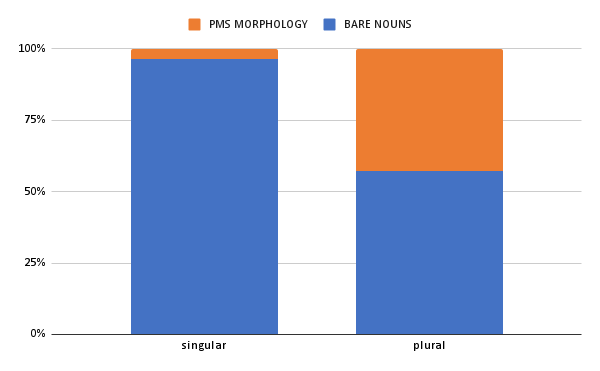
\includegraphics[width=\textwidth]{figures/GoriaBellamyChapter-img001.png}
\caption{Ratios of bare stems \textit{vs} inflected nouns in the singular and plural (\textsc{n}=236)}
\label{fig:goria:1}
\end{figure}

The picture becomes even clearer if we focus exclusively on plural nouns, which constitute the area where most variation is observed. Based on the distribution of \tabref{tab:goria:9}, we thus repeated Fisher’s exact test only on plural nouns in order to test the distribution for statistical significance. The test returned a \textit{p value} of 0.002, thus demonstrating that Spanish masculine nouns occur more frequently as bare stems in code-mixing, and are therefore treated as invariables, whereas feminine nouns are more frequently matched to the Piedmontese -\textit{a/-e} class, and thus are inflected with the Piedmontese plural marker \textit{{}-e}; see \figref{fig:goria:2}.

\begin{figure}
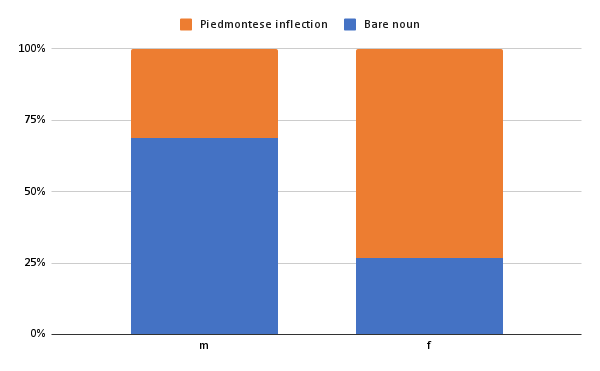
\includegraphics[width=\textwidth]{figures/GoriaBellamyChapter-img002.png}
\caption{Ratios of the two strategies of plural marking observed for masculine and feminine nouns (\textsc{n}=63)}
\label{fig:goria:2}
\end{figure}

\section{Discussion and conclusions}

The analysis of Spanish-Piedmontese code-mixing carried out in this study enabled us first of all to publish new data in English about a language, Piedmontese, that is endangered in its homeland and that is spoken in an even more fragile ecology in the post-migration setting of Argentina described in the previous sections. We therefore regard the present contribution as a milestone in the documentation of Heritage Piedmontese.

We were able to identify a number of tendencies that characterise the bilingual situation presented in this study, with the main aim of determining what type of code-mixing predominated among and between the speakers. To this end, the data revealed a much greater preference for insertion over alternation, which appears to be a marginal phenomenon in the corpus. This preference can be interpreted as a tendency towards what \citet{DalNegro2013} (see also \citealt{Clyne2003}) refers to as “intended monolingualism”, that is the choice to establish the heritage language as the base language of the interaction, and as the matrix language of the clause, thereby avoiding larger shifts towards Spanish, as is the case with alternation. As mentioned in \sectref{sec:goria:3}, the reason for this choice is probably an effect of the fact that speakers generally show positive attitudes towards \textsc{hp} and tend to position themselves as proficient speakers of the language, and therefore they tend to display their knowledge also by avoiding major switches to Spanish. Other evidence in favour of this view is given by the presence of self-corrections and feedback towards other speakers when too much Spanish was used in the conversation. At the same time, one of the most salient features in \textsc{hp} is indeed the abundant presence of Spanish lexicon that characterises code-mixing (as opposed to code-switching; see the discussion in 3.3): most of the evaluations collected on the field identify this phenomenon as one of the hallmarks of \textit{piemonteis merican,} that is the name given by the community to \textsc{hp}.

In contrast, a possible explanation for the observed distribution resides in the methodology used for data collection: since the data were collected with the primary purpose of documenting \textsc{hp}, the interviewer systematically used that language during data collection (see also the methodological remarks in \citealt{BlommaertDong2010}), thus inviting monolingual contributions in this language, and possibly preventing other conversational styles where alternation between Spanish and \textsc{hp} occurs more frequently. 

Quantitative analysis of noun insertion showed that maximal insertions represent a marginal phenomenon in the corpus compared to minimal insertions, which are the most frequent pattern. We then moved on to evaluate if, based on the typology of gender and number marking on nouns in the two contact languages, it was possible to predict the observed type of switch. The results seem to confirm our hypothesis: as a general consideration, we may conclude that at the points where the two languages are structurally equivalent, the same structure is maintained in code-mixing; and thus, although from a partially different theoretical perspective, we may observe that \citegen{Poplack1980} equivalence principle is well reflected in this data. The prevalence of bare nouns in the singular is best interpreted as a reflection of the fact that in both Spanish and Piedmontese singular number is zero-marked; in fact, most of the singular nouns that have overt Piedmontese morphemes are derived words such as \textit{chacar-é} ‘farmer’ (Spanish \textit{chacarero}), and \textit{alambr-à} ‘wiring’ (Spanish \textit{alambrado}), which obtain singular marking through the adoption of a Piedmontese derivational suffix.

Plural nouns, on the other hand, displayed more variation in code-mixing, with significant differences between masculine and feminine nouns. While the bare noun strategy is preferred for masculine nouns, feminines more frequently adopt Piedmontese overt morphology. Again, the Piedmontese number system provides an explanation for this difference, as masculine nouns are mostly invariables, whereas feminine nouns have overt inflection. Furthermore, this tendency may also be reinforced by a peculiarity of spoken Argentinian Spanish, as the plural marker \textit{{}-s} is involved in the phenomenon of phonetic reduction of syllable final \textit{{}-s}, with the effect of losing plural marking.

At the same time, we were able to identify a small number of cases of insertions that are not immediately predictable from the grammar of the two contact languages. We saw that some Spanish nouns are inserted into Piedmontese with a final /o/, both in the singular and in the plural, and in some cases, Spanish nouns in \textit{{}-e} take \textit{{}-i} as a plural marker in code-mixing. While the data are too scarce to make a more concrete claim, such instances might represent innovations that have arisen in the heritage language scenario and which have, at some point, diffused into the community, as they also appear in the first author’s field notes and in recordings that were not considered for this study. To conclude, this research supports the notion that identifying typological similarities and differences in the contact languages may indeed help us predict the type of code-mixing that will be observed. Thus, on the one hand the greater propensity for bare nouns seems to be determined by the fact that Spanish nouns are adapted to a grammatical frame where masculine nouns are invariables. Furthermore, we saw that if we take into account spoken Spanish, the equivalence is even greater due to phonetic reduction. Conversely, structural equivalence is also responsible for the presence of overtly inflected plural feminines, because a clearer match is found between Spanish and Piedmontese feminine nouns.

As a methodological note, it must also be observed that in this study we used as a benchmark for evaluating structural innovations in \textsc{hp} the written variety of Torino, which has provided a basis for grassroots revitalisation initiatives within the community (in Italy) and for grammatical description. This might be problematic in principle, as it could blur out internal variation in the input, which is – as is well known – one of the sources of language change in heritage languages. However, we must stress that none of the non-target forms that were identified in the dataset can be associated with any of the local dialects of Piedmontese. Internal variation in Piedmontese will need to be necessarily taken into account if this research is extended to other sectors of grammar were greater variation is observed (e.g. determiners).

Finally, the observation of this situation at the synchronic level of code-mixing also leads us to some observations about diachronic language change (see \citealt{Backus2005}). While we are not able to reconstruct how code-mixing was in the past and what the origins of this situation might be, we may ask whether the observed preference for bare nouns, at least in the masculine, may represent an emergent change in \textsc{hp}, especially on account of the observed overextensions such as Spanish \textit{balde} ‘bucket’ being realised as \textit{baldo.} Also the presence of emic identification of these forms as typical of \textsc{hp} seems to point in this direction. Such a hypothesis of course needs to be tested on a much larger dataset, also taking into consideration other factors such as internal variation in the community, the type of literacy that the speakers have in the heritage language, and so on. However, if supported, it could provide relevant evidence for the relation between code-mixing at the synchronic level and diachronic language change.


\sloppy\printbibliography[heading=subbibliography,notkeyword=this]
\end{document} 
